\documentclass{beamer}

\mode<presentation>{
\usetheme{Madrid}
%\usecolortheme{beaver}
}
\usepackage[utf8]{inputenc}
\usepackage{default}
\usepackage[portuguese]{babel}
\usepackage{pgfplots}
\pgfplotsset{/pgf/number format/use comma,compat=newest}
\usepackage{color}
\usepackage{amsmath,amsfonts,amssymb}
\usepackage{hyperref}
\usepackage{tikz}
% Para imagens
\usepackage{graphicx}
\usepackage{subcaption}
%\usepackage{float} % necessário para manter as imagens no lugar certo
%Para a tabela
%\usepackage{tabu}
%\usepackage{tabularx}
%\usepackage{multirow}


\usebackgroundtemplate{%
\tikz\node[opacity=0.05] {
\includegraphics[height=\paperheight,width=\paperwidth]{logo_IME.png}};}


\title[Energia em IoT]{Consumo de Energia e uso de Bateria em Projetos de Internet das Coisas}
\author[Marcelo Schmitt]{Marcelo Schmitt}
\institute[IME-USP]{Universidade de São Paulo}
%\date{\today}
\date{}

\begin{document}

\begin{frame}
 \maketitle
\end{frame}

\begin{frame}
\frametitle{Sumário}
 \tableofcontents
\end{frame}

\section{Introdução}
\begin{frame}
\frametitle{Introdução}
\begin{minipage}{\textwidth}

Muitos projetos de internet das coisas (IoT) usam placas de prototipagem rápida como Arduino e NodeMCU na sua implementação inicial. Contudo, pouca atenção se dá a forma como essas placas (e os componentes ligados a elas) são alimentados eletricamente. \\


Esta apresentação cobrirá os seguintes tópicos:
\begin{itemize}
	\item Principais placas de prototipagem rápida para IoT
	\begin{itemize}
		\item Um pouco mais sobre NodeMCU
	\end{itemize}
	\item Especifidades de alimentação elétrica para placas de IoT
	\item Opções de como energizar projetos de IoT
\end{itemize}

\end{minipage}
\end{frame}

\section{Principais Placas para IoT}


\begin{frame}
\frametitle{Principais Placas}
\begin{minipage}{\textwidth}
	
	\begin{figure}
		\centering
		\begin{subfigure}[b]{0.25\textwidth}
			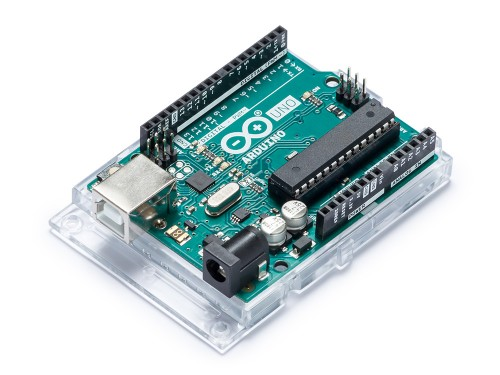
\includegraphics[width=\textwidth]{arduinoUNO.jpg}
			\caption{ArduinoUNO}
			\label{fig:arudinddfo_uno}
		\end{subfigure}
		\begin{subfigure}[b]{0.25\textwidth}
			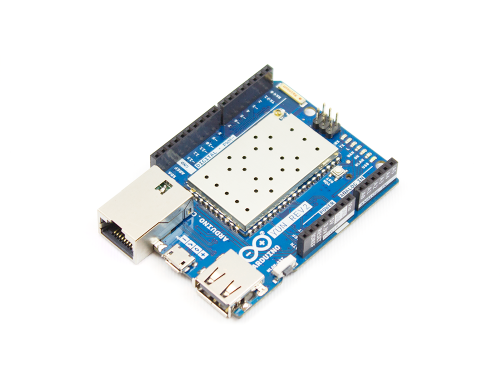
\includegraphics[width=\textwidth]{arduino_yun.png}
			\caption{Arduino Yun}
			\label{fig:node_mcudfd}
		\end{subfigure}
		\begin{subfigure}[b]{0.25\textwidth}
			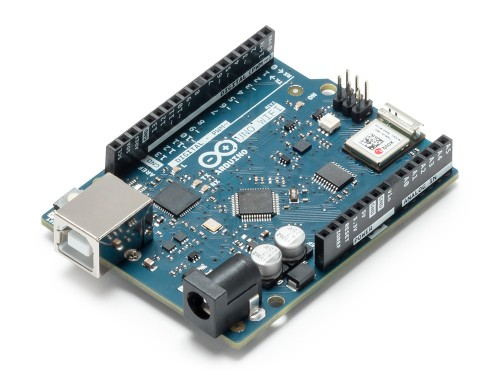
\includegraphics[width=\textwidth]{arduinoUNO_wifi.jpg}
			\caption{ArduinoUNO WiFi}
			\label{fig:nofdfdde_mfdfdcudfd}
		\end{subfigure}
		\caption{Placas da família Arduino}
		\label{fig:plfdacddsfa_iot}
		\vspace{-10pt}
	\end{figure}
	As placas da família Arduino tem boa documentação, uma ampla comunidade de usuários, e uma IDE amigável com programação semelhante a C/C++.
	
\end{minipage}
\end{frame}

\begin{frame}
	\frametitle{Principais Placas}
	\begin{minipage}{\textwidth}
		
		\begin{figure}
			\centering
			\begin{subfigure}[b]{0.25\textwidth}
				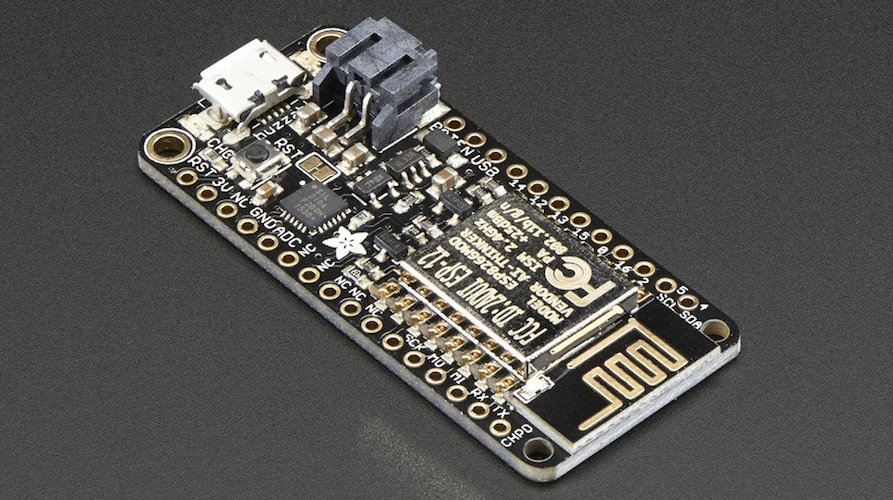
\includegraphics[width=\textwidth]{Feather_HUZZAH.jpg}
				\caption{Adafruit Feather Huzzah}
				\label{fig:arudifdnddfo_uno}
			\end{subfigure}
			\begin{subfigure}[b]{0.25\textwidth}
				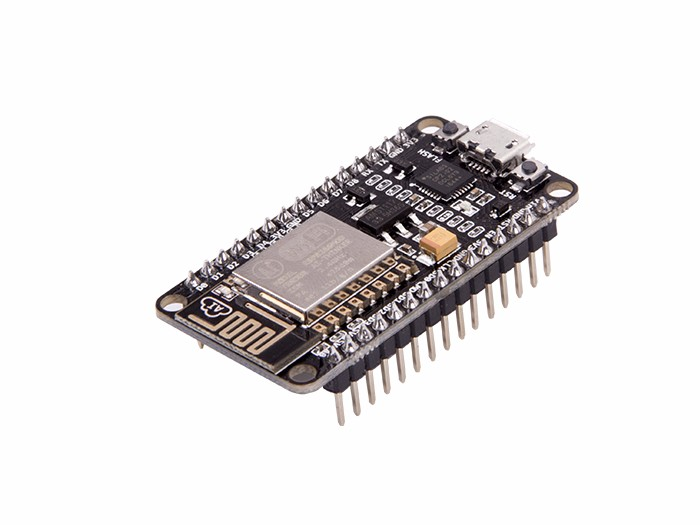
\includegraphics[width=\textwidth]{NodeMCUAmica.jpg}
				\caption{NodeMCU Amica}
				\label{fig:node_mdscudfd}
			\end{subfigure}
			\begin{subfigure}[b]{0.25\textwidth}
				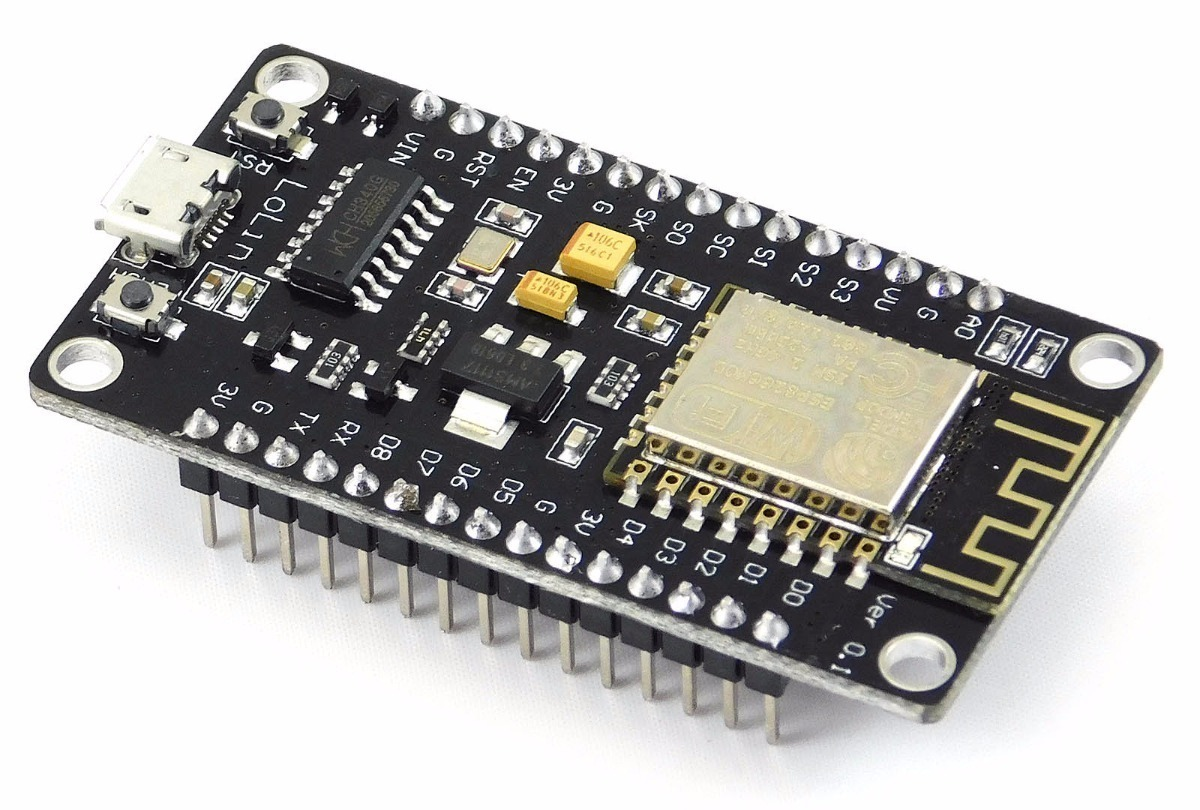
\includegraphics[width=\textwidth]{NodeMCUlolin.jpg}
				\caption{NodeMCU LoLin}
				\label{fig:nofdfdde_mfsddfdcudfd}
			\end{subfigure}
			
			\begin{subfigure}[b]{0.25\textwidth}
				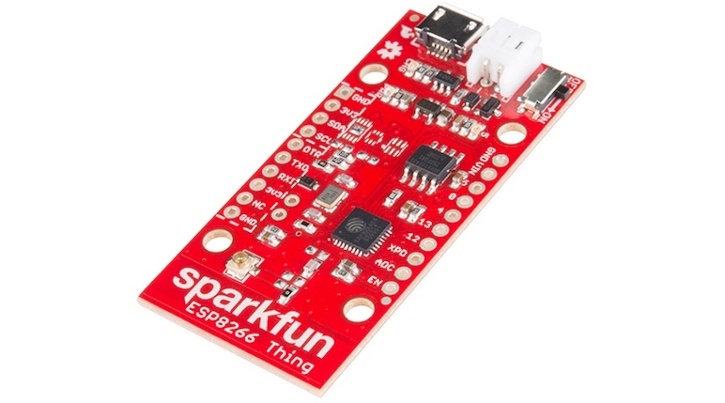
\includegraphics[width=\textwidth]{Sparkfun.jpg}
				\caption{SparkFun ESP8266 Thing}
				\label{fig:nofdfdde_mfsddfdcudfhfd}
			\end{subfigure}
			\begin{subfigure}[b]{0.25\textwidth}
				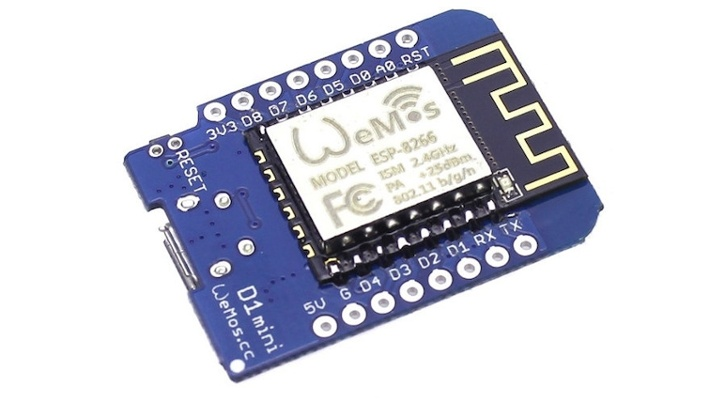
\includegraphics[width=\textwidth]{Wemos_D1_mini.jpg}
				\caption{WeMos D1 mini}
				\label{fig:nofdfdde_mfsddfdsfddcudfd}
			\end{subfigure}
			%~ %add desired spacing between images, e. g. ~, \quad, \qquad, \hfill etc. 
			%(or a blank line to force the subfigure onto a new line)
			\caption{Placas do tipo NodeMCU}
			\label{fig:placddsfa_iot}
			%\vspace{-20pt}
		\end{figure}
	\end{minipage}
\end{frame}


\begin{frame}
\frametitle{Um Pouco mais sobre NodeMCU}
\begin{minipage}{\textwidth}
	
	O NodeMCU (Node MicroController Unit) é um ambiente de desenvolvimento de software e hardware abertos construído sobre um SoC (Sistema em um Chip) de baixo custo chamdo ESP8266. O ESP8266 (ou ESP12), contém todos os elementos cruciais de um computador moderno: CPU, RAM, dispositivo de rede (wifi), um micro sistema operacional, e um SDK.\cite{node_mcu_acronimo}
	
	%The NodeMCU (Node MicroController Unit) is an open source software and hardware development environment that is built around a very inexpensive System-on-a-Chip (SoC) called the ESP8266. The ESP8266, designed and manufactured by Espressif Systems, contains all crucial elements of the modern computer: CPU, RAM, networking (wifi), and even a modern operating system and SDK. When purchased at bulk, the ESP8266 chip costs only \$2 USD a piece. That makes it an excellent choice for IoT projects of all kinds.
	%https://www.ibm.com/developerworks/library/iot-nodemcu-open-why-use/index.html	
	
	
	\begin{figure}
		\centering
		\vspace{-10pt}
		\begin{subfigure}[b]{0.25\textwidth}
			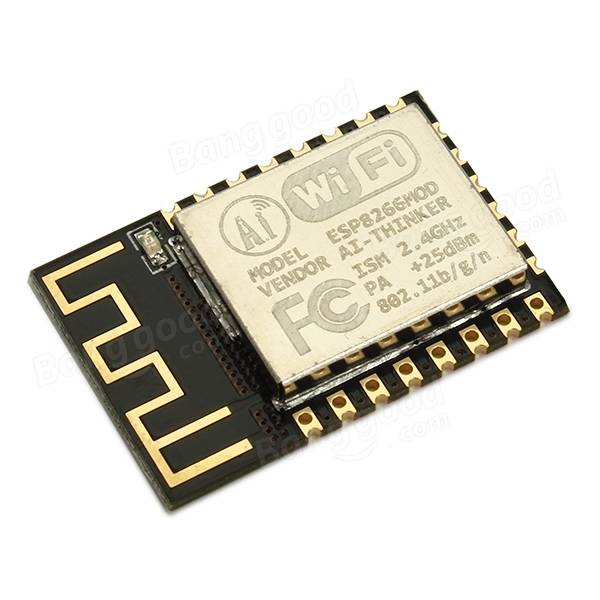
\includegraphics[width=\textwidth]{ESP8266AIThinker.jpg}
			\caption{ESP8266 AI Thinker}
			\label{fig:arudinddffgdo_uno}
		\end{subfigure}
		\begin{subfigure}[b]{0.25\textwidth}
			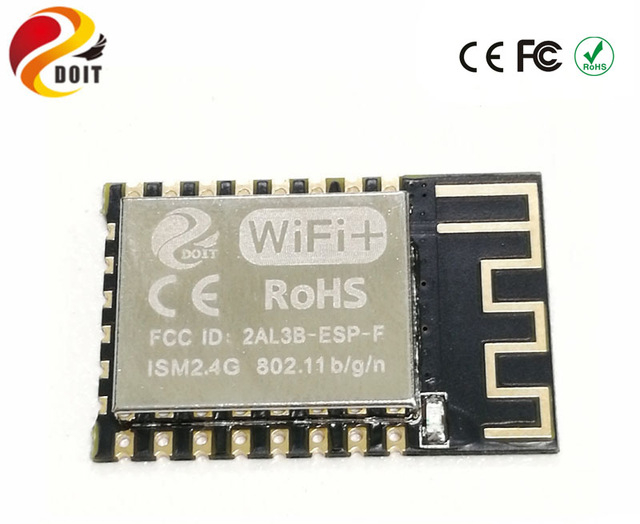
\includegraphics[width=\textwidth]{DOIT-ESP8266-ESP-F.jpg}
			\caption{ESP8266 DOIT}
			\label{fig:ndgdfode_mcudfd}
		\end{subfigure}
		\begin{subfigure}[b]{0.25\textwidth}
			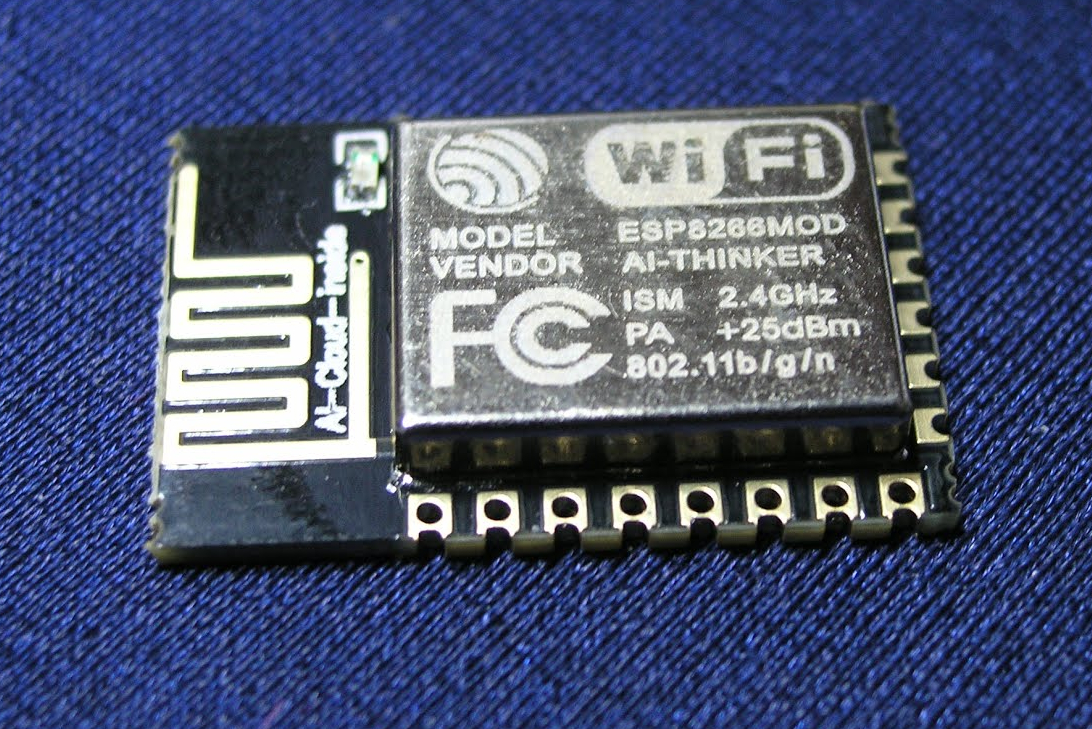
\includegraphics[width=\textwidth]{ESP8266Espressif.JPG}
			\caption{ESP8266 Espressif}
			\label{fig:nofdffgfgdde_mfdfdcudfd}
		\end{subfigure}
		\caption{ESP8266 de diferentes fabricantes}
		\label{fig:phghglfdacddsfa_iot}
		%\vspace{-10pt}
	\end{figure}

\end{minipage}
\end{frame} 

\begin{frame}
\frametitle{Quantas Versões de NodeMCU?}
\begin{minipage}{\textwidth}
	
	%What further contributes to the naming jungle is precisely the fact that the hardware is open-source and anyone can produce and market NoduMCU development boards. There currently are three primary producers: Amica (see ‘NodeMCU and Amica‘ below), DOIT/SmartArduino, and LoLin/WeMos.
	%https://frightanic.com/iot/comparison-of-esp8266-nodemcu-development-boards/#names
	%Generation	Version	“Common” Name
	%1st	0.9	V1
	%2nd	1.0	V2
	%2nd	1.0	V3
	
	%The following images compare the LoLin NodeMCU (v3) with an Amica NodeMCU (v2).
	%https://cknodemcu.wordpress.com/2015/11/13/nodemcu-variants/
	
	\begin{figure}
		\centering
		\begin{subfigure}[b]{0.25\textwidth}
			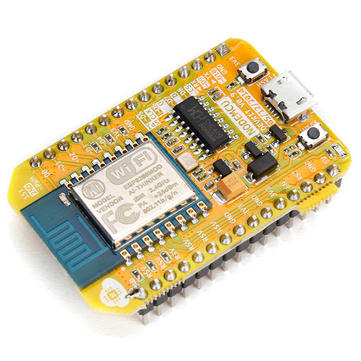
\includegraphics[width=\textwidth]{NodeMCU09.jpg}
			\caption{NodeMCU original}
			\label{fig:arudfdsidfsdno_uno}
		\end{subfigure}
		\begin{subfigure}[b]{0.25\textwidth}
			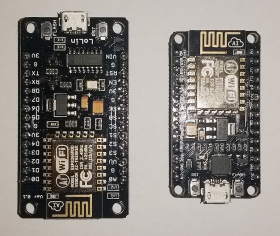
\includegraphics[width=\textwidth]{amica-vs-lolin-1.png}
			\caption{LoLin Vs Amica - visão de cima}
			\label{fig:arudfdsino_uno}
		\end{subfigure}
		~ %add desired spacing between images, e. g. ~, \quad, \qquad, \hfill etc. 
		%(or a blank line to force the subfigure onto a new line)
		\begin{subfigure}[b]{0.25\textwidth}
			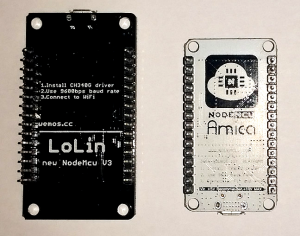
\includegraphics[width=\textwidth]{amica-vs-lolin-2.png}
			\caption{LoLin Vs Amica - visão de baixo}
			\label{fig:nodesdf_mcu}
		\end{subfigure}
		~ %add desired spacing between images, e. g. ~, \quad, \qquad, \hfill etc. 
		%(or a blank line to force the subfigure onto a new line)
		\caption{Principais modelos de NodeMCU}\label{fig:pfsdlaca_iot}
		\vspace{-20pt}
	\end{figure}
	
	\begin{center}
		\begin{tabular}{l|c|r}
			Geração & Versão & Nome comum \\
			\hline
			1ª & 0.9 & V1 \\
			\hline
			2ª & 1.0 & V2 \\
			\hline
			3ª & 1.0 & V3 \\
		\end{tabular}	
	\end{center} \cite{versoes_nodemcu}

\end{minipage}
\end{frame} 


\begin{frame}
\frametitle{Oficial Vs Não Oficial}
\begin{minipage}{\textwidth}
	
	Embora o domínio \url{www.nodemcu.com} pertença a empresa Amica, como o hardware é aberto qualquer um é livre para fabricar a sua versão de NodeMCU e portanto não faz muito sentido dizer que uma placa é "oficial". \cite{comparacao_placas_nodemcu} \cite{wemos}
	
	%Official vs Unofficial
	%NodeMCU posted a photo on Facebook which shows official and unofficial V2 boards. I don’t really understand the notion of official. It’s my understanding that with open-source hardware there’s no such thing as official boards. What it maybe means is that Amica is the “endorsed” producer and DOIT \& LoLin are not.
	
	%Wemos We use new logo "LOLIN" from 2017-04-25.
	%https://www.wemos.cc/
	
	% WEMOS is a young Chinese company, we designed lots of cost-effective IoT products. 
	%https://www.wemos.cc/
	
	\begin{figure}
		\centering
		\begin{subfigure}[b]{0.25\textwidth}
			
\includegraphics[width=\textwidth]{AmicaLogo.png}
			\caption{Amica}
			\label{fig:arudino_unsdfo}
		\end{subfigure}
		~ %add desired spacing between images, e. g. ~, \quad, \qquad, \hfill etc. 
		%(or a blank line to force the subfigure onto a new line)
		\begin{subfigure}[b]{0.2\textwidth}
			
\includegraphics[width=\textwidth]{versus.jpg}
			%\caption{WeMos / LoLin}
			\label{fig:nodsdfsde_mcudf}
		\end{subfigure}
		\begin{subfigure}[b]{0.25\textwidth}
			
\includegraphics[width=\textwidth]{WeMos.png}
			\caption{WeMos / LoLin}
			\label{fig:node_mcudf}
		\end{subfigure}
		~ %add desired spacing between images, e. g. ~, \quad, \qquad, \hfill etc. 
		%(or a blank line to force the subfigure onto a new line)
		\caption{Duas das principais fabricantes de placas chamadas NodeMCU}\label{fig:placa_sdfsiot}
		\vspace{-20pt}
	\end{figure}
	
	
\end{minipage}
\end{frame} 



\section{Especifidades de alimentação elétrica para placas de IoT}


\begin{frame}
\frametitle{Especificações elétricas}
\begin{minipage}{\textwidth}
	
		\begin{figure}[!ht]
			\centering
			
\includegraphics[width=0.9\textwidth]{menino-choque.jpg}
			%\caption{}
			\label{fig:ndfgodsdfsde_power_pins}
			\vspace{-10pt}
		\end{figure}

\end{minipage}
\end{frame} 


\begin{frame}
\frametitle{Família Arduino}
\begin{minipage}{\textwidth}
	\begin{itemize}
		\item ArduinoUNO: Voltagem de alimentação 7-12V\cite{arduino-uno}  (recomendado), consumo de corrente elétrica de aproximadamente 25mA\cite{arduino_forum1} em modo ativo.
		\item Arduino Yun: Voltagem de alimentação 7-12V, consumo de corrente elétrica entre 170 e 250mA\cite{arduino_forum2} .
		
		%Even at it's lowest power measured (170ma) 
		%Tested yesterday with wifi enabled:
		%250mA @ 5V = 1.25
		%https://forum.arduino.cc/index.php?topic=188821.0
	\end{itemize}
\end{minipage}
\end{frame} 



%Arduino
%Active Mode: 0.2 mA
%Input Voltage (recommended) 7-12V
%https://store.arduino.cc/arduino-uno-rev3
%http://forum.arduino.cc/index.php?topic=5536.0


%ArduinoYun
%Even at it's lowest power measured (170ma) 
%Tested yesterday with wifi enabled:
%250mA @ 5V = 1.25
%https://forum.arduino.cc/index.php?topic=188821.0


\begin{frame}
	\frametitle{Família Arduino}
	\begin{minipage}{\textwidth}
		\begin{figure}[!ht]
			\centering
			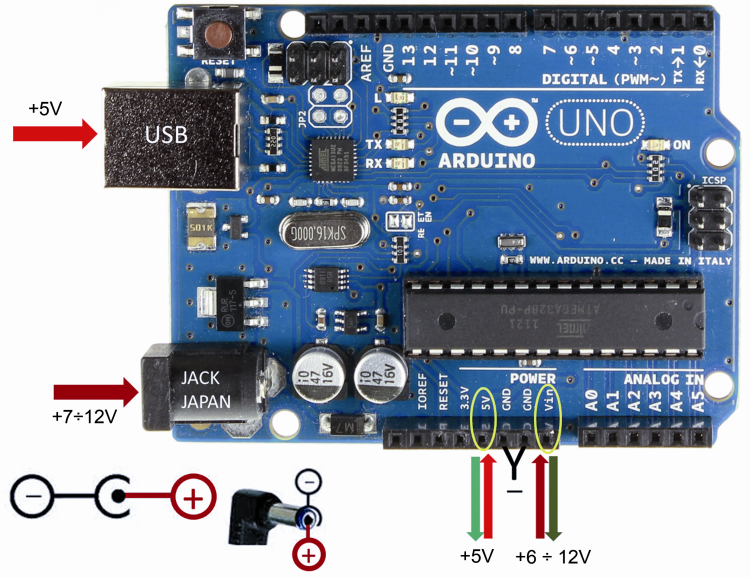
\includegraphics[width=0.6\textwidth]{arduino_power_pinout.png}
			\caption{Diagrama de pinos relacionados a alimentação elétrica do Arduino}
			\label{fig:ndfgode_power_pins}
			\vspace{-10pt}
		\end{figure}
		
	\end{minipage}
\end{frame} 


%NodeMCU amica
% Max Current: 1000mA
% Max Supply Voltage: 3.3-20V
%https://github.com/nodemcu/nodemcu-devkit-v1.0/blob/master/NODEMCU_DEVKIT_V1.0.PDF

% ESP-8266EX
% 170mA
% 



%spark fun
%https://cdn.sparkfun.com/datasheets/Wireless/WiFi/ESP8266ThingV1.pdf
%Transmit 135-215mA
%Receive 60-62mA
%Standby 0.9mA
%Deep sleep 10uA

%placa adafruit
%We use this to power the ESP8266 which can draw spikes of 250+mA
%We use a 500mA peak low-dropout regulator
%https://learn.adafruit.com/adafruit-feather-huzzah-esp8266/power-management
%https://cdn-learn.adafruit.com/downloads/pdf/adafruit-feather-huzzah-esp8266.pdf


\begin{frame}
\frametitle{Placas NodeMCU}
\begin{minipage}{\textwidth}
	
	\begin{itemize}
		\item Adafruit Feather Huzzah:  Voltagem de alimentação 5V (entrada USB), consumo médio de corrente elétrica de 500mA.\cite{adafruit-feather}
		
		\item SparkFun ESP8266 Thing: Voltagem de alimentação 3.3-5.5V, consumo médio de corrente elétrica de 500mA.\cite{sparkfunthing}
		
		\item NodeMCU (Amica e LoLin): Voltagem de alimentação 3.3-20V (dependente da entrada), consumo médio de corrente elétrica de 1000mA em modo ativo.\cite{nodemcu_amica_datasheet}
	\end{itemize}
	
	%NodeMCU
	%170 mA em modo ativo (pico de até 320mA na inicialização seguna fórum)
	
	%https://www.esp8266.com/viewtopic.php?f=13&t=3875
	%https://www.espressif.com/sites/default/files/documentation/0a-esp8266ex_datasheet_en.pdf
	%https://www.kloppenborg.net/images/blog/esp8266/esp8266-esp12e-specs.pdf

	%https://forum.arduino.cc/index.php?topic=445538.0

\end{minipage}
\end{frame}

\begin{frame}
	\frametitle{Especificidades do NodeMCU}
	\begin{minipage}{\textwidth}
		
		\begin{figure}[!ht]
			\centering
			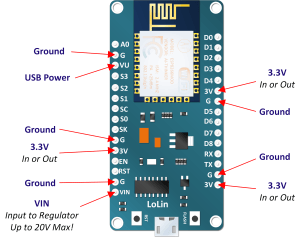
\includegraphics[width=0.4\textwidth]{ESP12-E-Developer-Board-Power-Pinouts.png}
			\caption{Diagrama de pinos relacionados a alimentação elétrica do NodeMCU LoLin V3}
			\label{fig:node_power_pins}
			\vspace{-10pt}
		\end{figure}
		
		\color{red}Importante: \color{black} Placas de outros fabricantes podem ter especificações diferentes. Sempre procure por informações dos componentes presentes na placa que você tem em mãos.
		
	\end{minipage}
\end{frame} 


\section{Opções de Alimentação}

\begin{frame}
\frametitle{Opções para Alimentar Projeto de IoT}
\begin{minipage}{\textwidth}
	\begin{figure}[!ht]
		\centering
		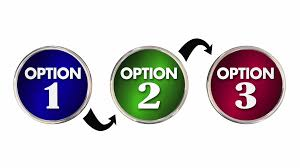
\includegraphics[width=0.8\textwidth]{opcoes.jpeg}
		%\caption{Diagrama de pinos relacionados a alimentação elétrica do ArduinoUNO}
		\label{fig:ndfgode_dfgdpodsdswer_pins}
		\vspace{-10pt}
	\end{figure}
	
	%battery-super-man.jpg
\end{minipage}
\end{frame} 

\begin{frame}
	\frametitle{Opções para Alimentar Placas Arduino}
	\begin{minipage}{\textwidth}
		\begin{figure}[!ht]
			\centering
			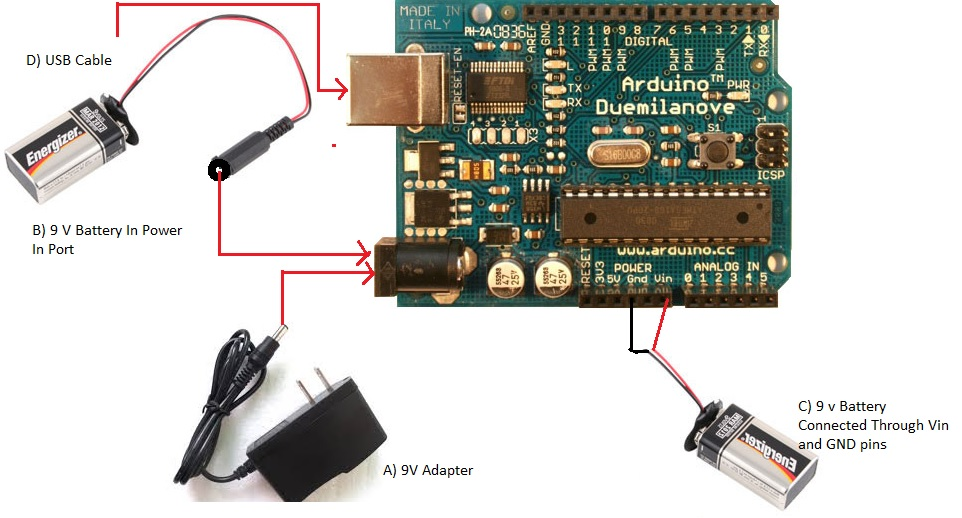
\includegraphics[width=0.6\textwidth]{alimentacao_ArduinoUNO.jpg}
			\caption{Alguns modos de alimentar um Arduino}
			\label{fig:ndfgode_dfgdpower_pins}
			\vspace{-10pt}
		\end{figure}
	\end{minipage}
\end{frame} 



\begin{frame}
\frametitle{Opções para Alimentar Placas NodeMCU}
\begin{minipage}{\textwidth}
	Três principais formas de alimentar eletricamente um NodeMCU:
	
	\begin{itemize}
		\item
		Alimentação por USB: Opção padrão durante o desenvolvimento pois permite fazer upload de programas para o NodeMCU. 
		%Use USB Power   Great for loading programs,  but not so good if you want to actually have your project disconnected from the computer.
		\item 
		Fornecer 3V por um dos pinos de 3.3V: Posibilita o uso de fontes e reguladores de tensão para prover uma alimentação elétrica mais estável.
		%Provide 3.3V directly  This is a strong option.  With your own off board regulator,  you can provide a robust power source for your device.
		\item
		Alimentação pelo pino VIN: Fornecendo energia pelo pino VIN o regulador de tensão pode suprir até 800mA de corrente para a placa. Na maioria dos casos isso é suficiente para alimentar um série de sensores. Deve-se tomar cuidado quando alimentar outros dispositivos usando pinos de 3.3V.
		%Provide Power to VIN   The regulator is rated up to 800 mA.   In may cases, that is more than sufficient.   Care should be taken to keep track of your load if your intent is to power other devices from the 3.3.V pin.
		
	\end{itemize}
\end{minipage}
\end{frame} 

\begin{frame}
\frametitle{Cabo USB}
\begin{minipage}{\textwidth}
	\begin{figure}[!ht]
		\centering
		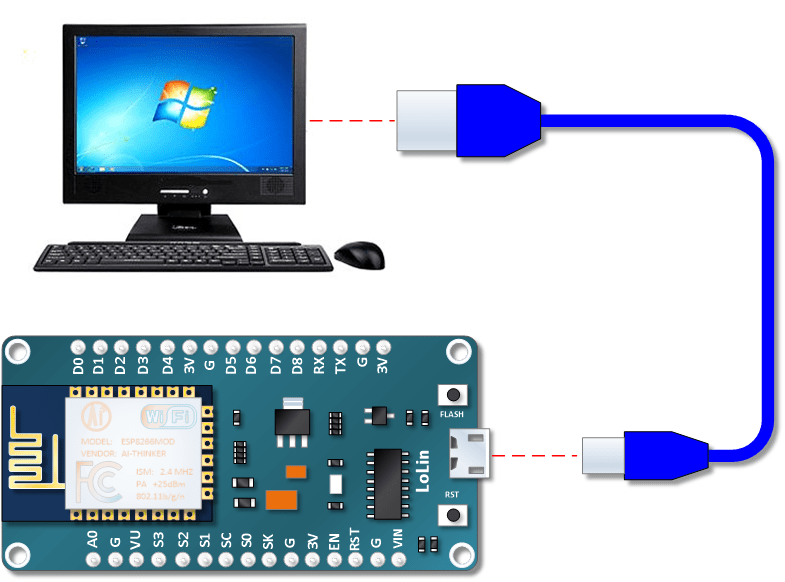
\includegraphics[width=0.4\textwidth]{Connect-to-Computer.png}
		\caption{NodeMCU ligado a um computador}
		\label{fig:alimentacao_usb}
	\end{figure}
\end{minipage}

Funciona para a maioria das placas e sistemas operacionais. \\
Podem ocorrer problemas de compatibilidade com MAC\footnote{\url{https://github.com/nodemcu/nodemcu-devkit-v1.0/issues/4}}.

\end{frame} 

\begin{frame}
\frametitle{Fonte de Bancada - Fonte de Protoboard}
\begin{minipage}{\textwidth}
	\begin{figure}
		\centering
		\begin{subfigure}[b]{0.4\textwidth}
			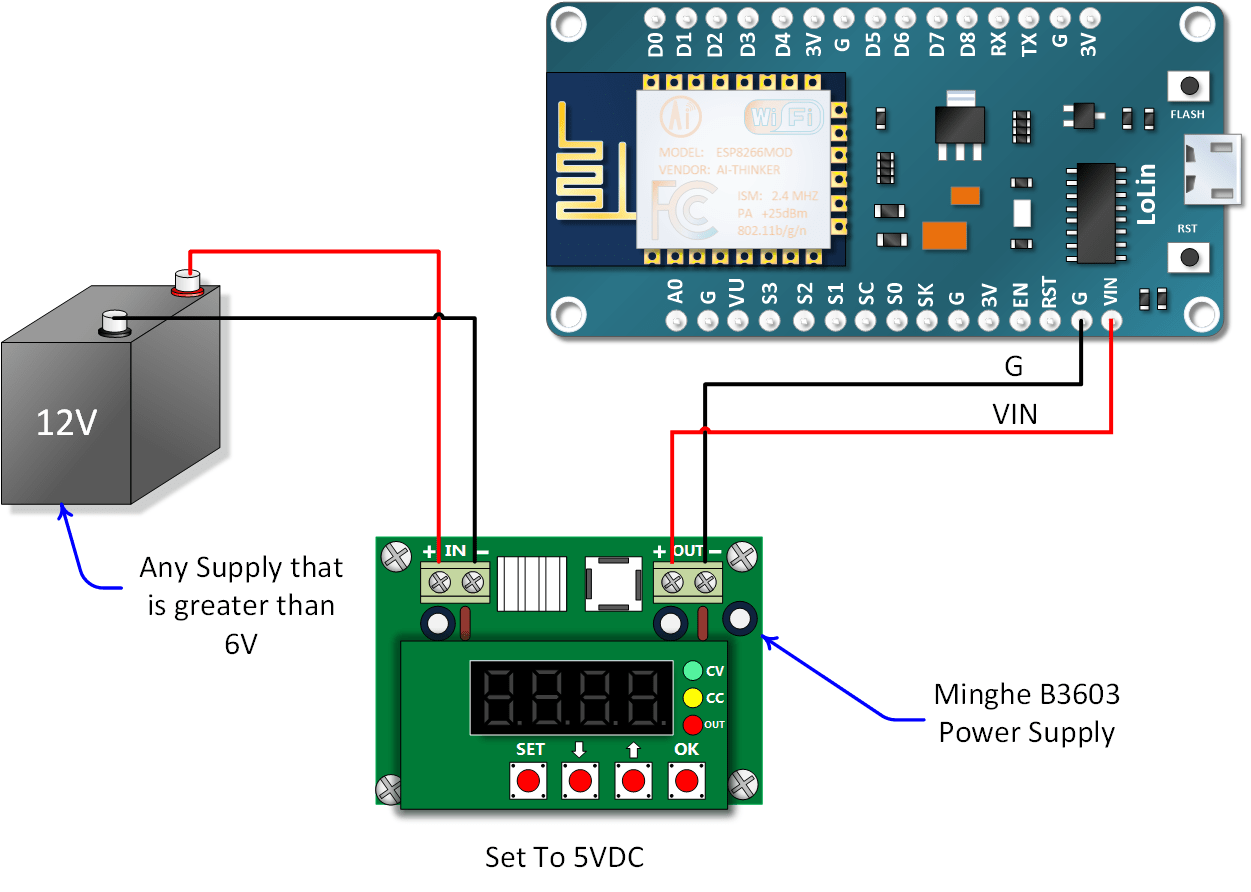
\includegraphics[width=\textwidth]{NodeMCU-Powered-by-B3603.png}
			\caption{Esquemático}
			\label{fig:arudinofdfd_uno}
		\end{subfigure}
		~ %add desired spacing between images, e. g. ~, \quad, \qquad, \hfill etc. 
		%(or a blank line to force the subfigure onto a new line)
		\begin{subfigure}[b]{0.25\textwidth}
			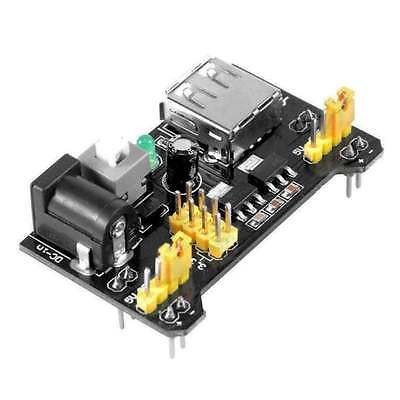
\includegraphics[width=\textwidth]{fonte_protoboard.jpg}
			\caption{Fonte de protoboard}
			\label{fig:nodefdf_mcu}
		\end{subfigure}
		~ %add desired spacing between images, e. g. ~, \quad, \qquad, \hfill etc. 
		%(or a blank line to force the subfigure onto a new line)
		\caption{Alimentação com fontes de bancada / protoboard}\label{fig:placa_dfdiot}
		\vspace{-20pt}
	\end{figure}
	Uma configuração semelhante ao esquema acima pode ser utilizada. Basta configurar a voltagem de saída da fonte de alimentação para 3.3V e conectá-la a um dos pinos de 3.3V da placa.
	
	%A set up similar to what is pictured above is what will be required.  Set the voltage to 3.3 Volts and connect to one of the 3V inputs.
\end{minipage}
\end{frame} 


\begin{frame}
\frametitle{Fonte de Bancada - Fonte de Protoboard}
\begin{minipage}{\textwidth}
	\begin{figure}[!ht]
		\centering
		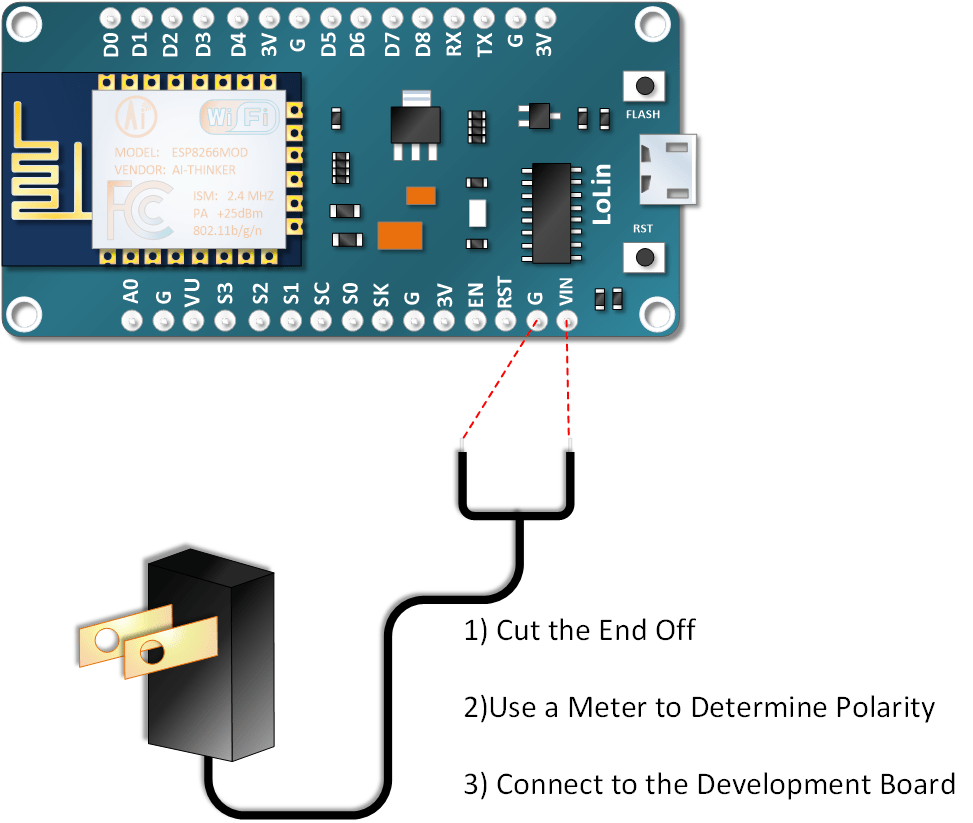
\includegraphics[width=0.4\textwidth]{ESP-12E-Powered-by-Wall-Wart.png}
		\caption{NodeMCU alimentado com uma fonte convencional}
		\label{fig:aligfgfmentacdffdao_usb}
	\end{figure}
	
	Pode ser usada uma fonte comum de 9V por exemplo. Basta cortar os fios de saída e ligá-los aos pinos de VIN e GND. Importante verificar a polaridade antes de fazer as ligações.
	%Something like a nine volt supply will work fine.   You just need to cut the end off.   Use a meter to verify polarity and then connect.
\end{minipage}
\end{frame} 

\begin{frame}
\frametitle{Bateria}
\begin{minipage}{\textwidth}
	\begin{figure}[!ht]
		\centering
		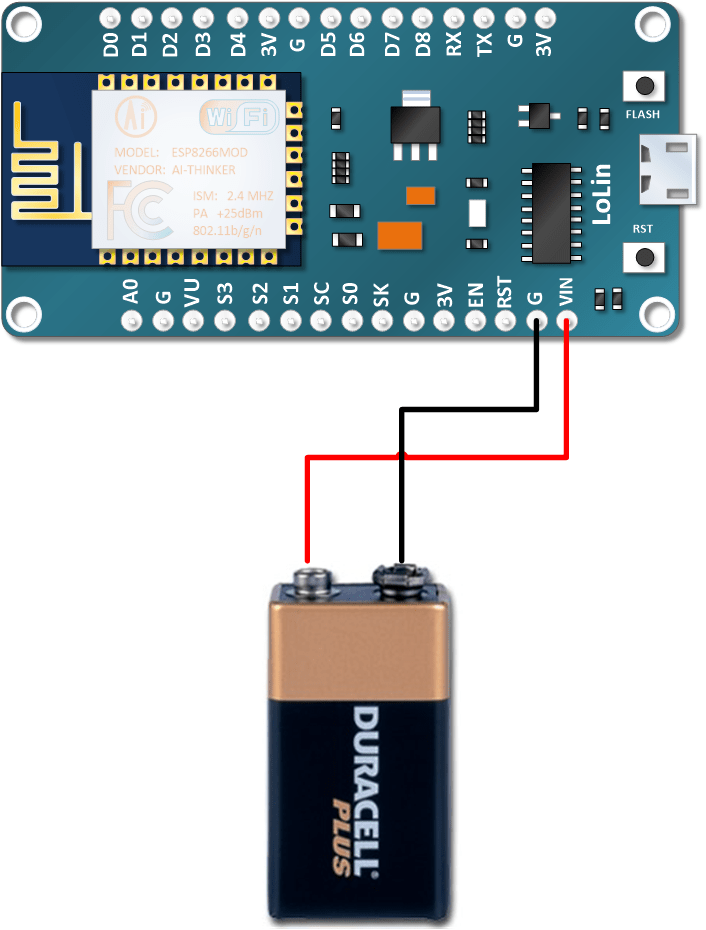
\includegraphics[width=0.2\textwidth]{Power-ESP-12E-with-a-9V-Battery.png}
		\caption{NodeMCU alimentado por uma bateria de 9V}
		\label{fig:aligfgfmentacdffdaodffdg_usb}
	\end{figure}
	Opção fácil e rápida mas de pouca duração. Outros tipos de bateria também podem ser utilizadas como a LiPo, li-ion, AAA (pilha palito), etc.
	
	Baterias recarregáveis podem tornar essa opção menos desencorajadora.
	%You may wish to think about re-chargeable batteries if this is the route you choose to go.
\end{minipage}
\end{frame} 

\begin{frame}
	\frametitle{Regulador de Tensão}
	\begin{minipage}{\textwidth}
		\begin{figure}[!ht]
			\centering
			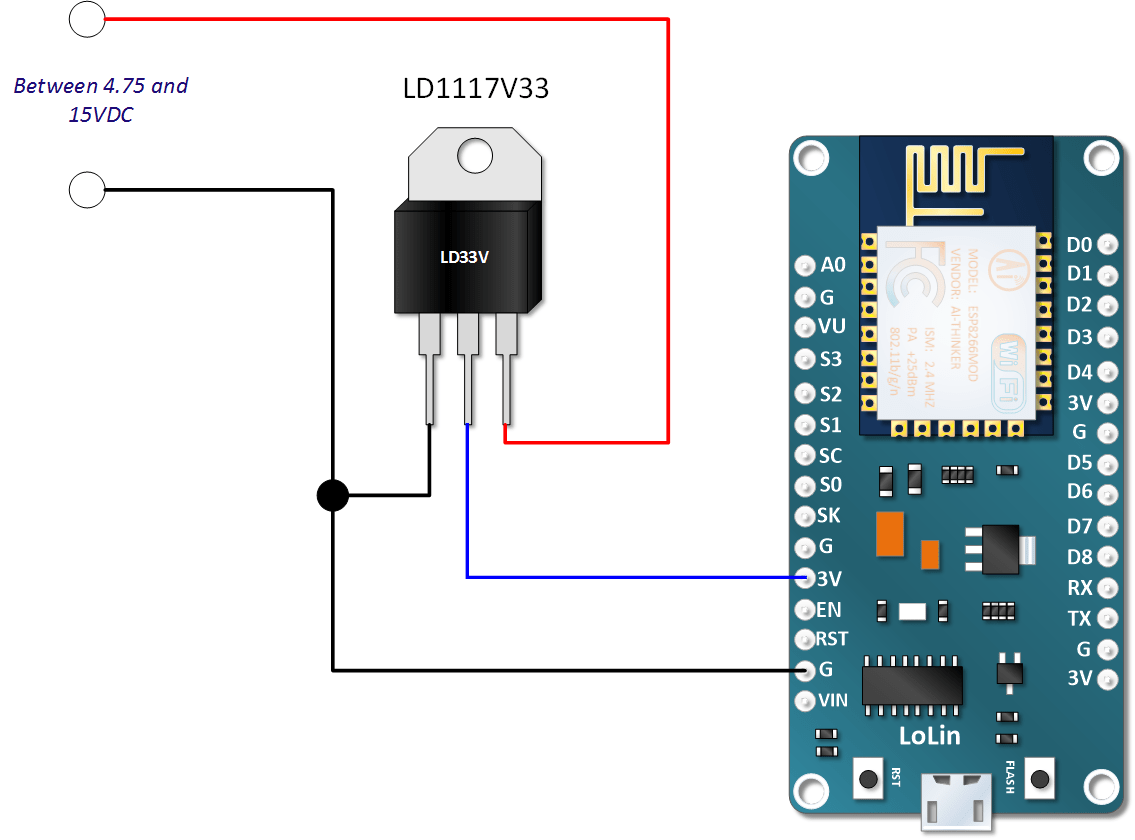
\includegraphics[width=0.4\textwidth]{Power-NodeMCU-with-LD33.png}
			\caption{NodeMCU alimentado com uso de um regulador de tensão}
			\label{fig:aligfgfmentacfdfddffdaodffdg_usb}
		\end{figure}
		Esta opão permite alimentar diretamente dispositivos de 3.3V. 
		
		%This option allows you to power other 3.3 volt devices.   I’d normally use some 10 uF capacitors in a circuit like this.   I didn’t find them necessary at the output because the NodeMCU board already has one.
	\end{minipage}
\end{frame} 


\section{Simulação de Consumo/Durabilidade de Baterias}

\begin{frame}
	\frametitle{Simulação de Consumo/Durabilidade de Baterias}
	\begin{minipage}{\textwidth}
		\begin{figure}[!ht]
			\centering
			
\includegraphics[width=0.8\textwidth]{battery-super-man.jpg}
			%\caption{Diagrama de pinos relacionados a alimentação elétrica do ArduinoUNO}
			\label{fig:ndfsdfsdgode_dfgdpodsdswer_pins}
			\vspace{-10pt}
		\end{figure}
		
	\end{minipage}
\end{frame} 


\begin{frame}
	\frametitle{Durabilidade em Modo Ativo}
	\begin{minipage}{\textwidth}
		\begin{figure}[!ht]
			\centering
			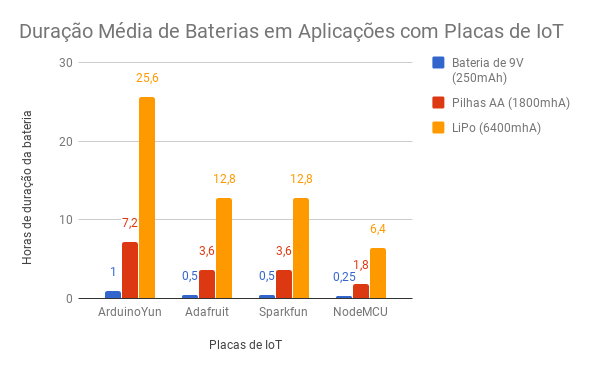
\includegraphics[width=0.9\textwidth]{duracao_modo_ativo.png}
			\caption{Gráfico de duração média de deferentes baterias quando usadas por placas IoT em modo ativo de operação.}
			\label{fig:ndfgode_podsfsdwer_pins}
			%\vspace{-10pt}
		\end{figure}
		
	\end{minipage}
\end{frame} 

%\begin{frame}
%	\frametitle{Durabilidade em Modo Econômico}
%	\begin{minipage}{\textwidth}
%		\begin{figure}[!ht]
%			\centering
%			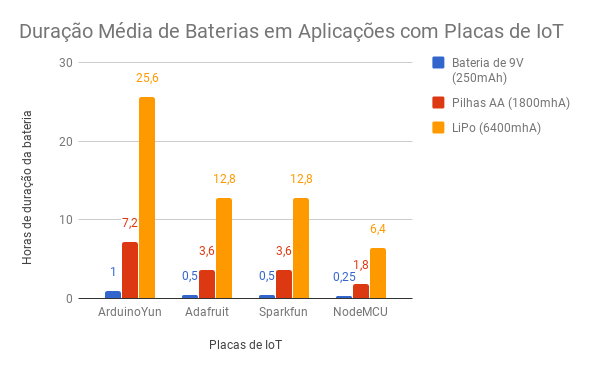
\includegraphics[width=0.9\textwidth]{duracao_modo_ativo.png}
%			\caption{Diagrama de pinos relacionados a alimentação elétrica do Arduino}
%			\label{fig:ndfgode_podssdfsdfsdwer_pins}
%			\vspace{-10pt}
%		\end{figure}
%		
%	\end{minipage}
%\end{frame} 

\section{Conclusão}

\begin{frame}
	\frametitle{Qual Placa Escolher?}
	\begin{minipage}{\textwidth}
		Depende ...
		\begin{itemize}
			\item do(s) sensor(es) e/ou atuador(es) a ser(em) utilizado(os)
			\item da fonte de alimentação
			\item da plataforma que será usada para o desenvolvimento
			\item do dinheiro disponível
			\item outros motivos ...
		\end{itemize}
	\end{minipage}
\end{frame} 

\section{Referências}
\begin{frame}
\frametitle{Referências}
\begin{thebibliography}{5}
	%\bibitem{beamer} \emph{Tantau T., Wright J. and Mileti\'{c} V. The BEAMER class - User Guide for version 3.36, March 2015}.
	%\bibitem{beamer2} \emph{Mertz A. and Slough W. Beamer by Example. The Prac\TeX~ Journal, n. 4, 2005.}
	%\bibitem{beamer1} \emph{Mohammad, et al.Machine Learning for Internet of Things Data Analysis - A Survey. Disponível em: \url{Suveri https://arxiv.org/pdf/1802.06305.pdf}}
	%\bibitem{beamer2} \emph{A. Mostafa, Yaser. - Learning From Data. Disponível em: \url{http://www.youtube.com/watch?v=FIbVs5GbBlQ&hd=1}}
	
	%\bibitem{beamer4} \emph{\url{https://en.wikipedia.org/wiki/Naive\_Bayes\_classifier}}

	
	\bibitem{node_mcu_acronimo}\href{https://www.ibm.com/developerworks/library/iot-nodemcu-open-why-use/index.html} {Getting to know NodeMCU and its DEVKIT board}
	
	\bibitem{versoes_nodemcu}\href{https://cknodemcu.wordpress.com/2015/11/13/nodemcu-variants/} {NodeMCU Variants}
	
	\bibitem{comparacao_placas_nodemcu} \href{https://frightanic.com/iot/comparison-of-esp8266-nodemcu-development-boards/}{Comparison of ESP8266 NodeMCU development boards}
	
	\bibitem{wemos} \href{https://www.wemos.cc/}{WeMos.cc}
	
	\bibitem{arduino-uno}\href{https://store.arduino.cc/arduino-uno-rev3} {Arduino-uno-rev3}
	
	\bibitem{arduino_forum1}\href{http://forum.arduino.cc/index.php?topic=5536.0}{Power Consumption Arduino - Fórum de Arduino}
	
	\bibitem{arduino_forum2}\href{https://forum.arduino.cc/index.php?topic=188821.0} {Arduino Yun, power draw - Fórum de Arduino}

	\bibitem{adafruit-feather}\href{https://cdn-learn.adafruit.com/downloads/pdf/adafruit-feather-huzzah-esp8266.pdf}{Adafruit Feather Huzzah - Datasheet}

	\bibitem{sparkfunthing}\href{https://cdn.sparkfun.com/datasheets/Wireless/WiFi/ESP8266ThingV1.pdf}{ESP8266Thing - Datasheet}
	
	\bibitem{nodemcu_amica_datasheet}\href{https://github.com/nodemcu/nodemcu-devkit-v1.0/blob/master/NODEMCU_DEVKIT_V1.0.PDF}{NodeMCU Amica - Datasheet}
	

	%\bibitem{espressif}\href{https://www.espressif.com/sites/default/files/documentation/0a-esp8266ex_datasheet_en.pdf}{ESP8266EX - Datasheet}


\end{thebibliography}

\end{frame}

\end{document}
